\documentclass[twoside]{book}

% Packages required by doxygen
\usepackage{fixltx2e}
\usepackage{calc}
\usepackage{doxygen}
\usepackage{graphicx}
\usepackage[utf8]{inputenc}
\usepackage{makeidx}
\usepackage{multicol}
\usepackage{multirow}
\PassOptionsToPackage{warn}{textcomp}
\usepackage{textcomp}
\usepackage[nointegrals]{wasysym}
\usepackage[table]{xcolor}

% Font selection
\usepackage[T1]{fontenc}
\usepackage{mathptmx}
\usepackage[scaled=.90]{helvet}
\usepackage{courier}
\usepackage{amssymb}
\usepackage{sectsty}
\renewcommand{\familydefault}{\sfdefault}
\allsectionsfont{%
  \fontseries{bc}\selectfont%
  \color{darkgray}%
}
\renewcommand{\DoxyLabelFont}{%
  \fontseries{bc}\selectfont%
  \color{darkgray}%
}
\newcommand{\+}{\discretionary{\mbox{\scriptsize$\hookleftarrow$}}{}{}}

% Page & text layout
\usepackage{geometry}
\geometry{%
  a4paper,%
  top=2.5cm,%
  bottom=2.5cm,%
  left=2.5cm,%
  right=2.5cm%
}
\tolerance=750
\hfuzz=15pt
\hbadness=750
\setlength{\emergencystretch}{15pt}
\setlength{\parindent}{0cm}
\setlength{\parskip}{0.2cm}
\makeatletter
\renewcommand{\paragraph}{%
  \@startsection{paragraph}{4}{0ex}{-1.0ex}{1.0ex}{%
    \normalfont\normalsize\bfseries\SS@parafont%
  }%
}
\renewcommand{\subparagraph}{%
  \@startsection{subparagraph}{5}{0ex}{-1.0ex}{1.0ex}{%
    \normalfont\normalsize\bfseries\SS@subparafont%
  }%
}
\makeatother

% Headers & footers
\usepackage{fancyhdr}
\pagestyle{fancyplain}
\fancyhead[LE]{\fancyplain{}{\bfseries\thepage}}
\fancyhead[CE]{\fancyplain{}{}}
\fancyhead[RE]{\fancyplain{}{\bfseries\leftmark}}
\fancyhead[LO]{\fancyplain{}{\bfseries\rightmark}}
\fancyhead[CO]{\fancyplain{}{}}
\fancyhead[RO]{\fancyplain{}{\bfseries\thepage}}
\fancyfoot[LE]{\fancyplain{}{}}
\fancyfoot[CE]{\fancyplain{}{}}
\fancyfoot[RE]{\fancyplain{}{\bfseries\scriptsize Generated on Sat Mar 19 2016 01\+:10\+:04 for Good Gob by Doxygen }}
\fancyfoot[LO]{\fancyplain{}{\bfseries\scriptsize Generated on Sat Mar 19 2016 01\+:10\+:04 for Good Gob by Doxygen }}
\fancyfoot[CO]{\fancyplain{}{}}
\fancyfoot[RO]{\fancyplain{}{}}
\renewcommand{\footrulewidth}{0.4pt}
\renewcommand{\chaptermark}[1]{%
  \markboth{#1}{}%
}
\renewcommand{\sectionmark}[1]{%
  \markright{\thesection\ #1}%
}

% Indices & bibliography
\usepackage{natbib}
\usepackage[titles]{tocloft}
\setcounter{tocdepth}{3}
\setcounter{secnumdepth}{5}
\makeindex

% Hyperlinks (required, but should be loaded last)
\usepackage{ifpdf}
\ifpdf
  \usepackage[pdftex,pagebackref=true]{hyperref}
\else
  \usepackage[ps2pdf,pagebackref=true]{hyperref}
\fi
\hypersetup{%
  colorlinks=true,%
  linkcolor=blue,%
  citecolor=blue,%
  unicode%
}

% Custom commands
\newcommand{\clearemptydoublepage}{%
  \newpage{\pagestyle{empty}\cleardoublepage}%
}


%===== C O N T E N T S =====

\begin{document}

% Titlepage & ToC
\hypersetup{pageanchor=false,
             bookmarks=true,
             bookmarksnumbered=true,
             pdfencoding=unicode
            }
\pagenumbering{roman}
\begin{titlepage}
\vspace*{7cm}
\begin{center}%
{\Large Good Gob }\\
\vspace*{1cm}
{\large Generated by Doxygen 1.8.8}\\
\vspace*{0.5cm}
{\small Sat Mar 19 2016 01:10:04}\\
\end{center}
\end{titlepage}
\clearemptydoublepage
\tableofcontents
\clearemptydoublepage
\pagenumbering{arabic}
\hypersetup{pageanchor=true}

%--- Begin generated contents ---
\chapter{Data Structure Index}
\section{Data Structures}
Here are the data structures with brief descriptions\+:\begin{DoxyCompactList}
\item\contentsline{section}{\hyperlink{structraygan__general__object}{raygan\+\_\+general\+\_\+object} }{\pageref{structraygan__general__object}}{}
\end{DoxyCompactList}

\chapter{File Index}
\section{File List}
Here is a list of all documented files with brief descriptions\+:\begin{DoxyCompactList}
\item\contentsline{section}{\hyperlink{gob_8c}{gob.\+c} }{\pageref{gob_8c}}{}
\item\contentsline{section}{\hyperlink{gob_8h}{gob.\+h} }{\pageref{gob_8h}}{}
\end{DoxyCompactList}

\chapter{Data Structure Documentation}
\hypertarget{structraygan__general__object}{\section{raygan\+\_\+general\+\_\+object Struct Reference}
\label{structraygan__general__object}\index{raygan\+\_\+general\+\_\+object@{raygan\+\_\+general\+\_\+object}}
}


{\ttfamily \#include $<$gob.\+h$>$}

\subsection*{Data Fields}
\begin{DoxyCompactItemize}
\item 
void $\ast$ \hyperlink{structraygan__general__object_aa8f4b6b7ad65fa40342f28c9ce30cb6b}{prev}
\item 
void $\ast$ \hyperlink{structraygan__general__object_abca7656e199e85edfa1304150cb2d7d9}{next}
\item 
void $\ast$ \hyperlink{structraygan__general__object_a571269e726fb52755234c73b02ad9ea8}{prevgarb}
\item 
void $\ast$ \hyperlink{structraygan__general__object_a97be0f07a3b6afe858c5c6ba8f3e1987}{nextgarb}
\item 
void($\ast$ \hyperlink{structraygan__general__object_aa4c5799d4485b20618b80d670c55b598}{cleanup} )(void $\ast$)
\end{DoxyCompactItemize}


\subsection{Detailed Description}
Subclass this object by making it the first data field in a structure or by making a subclass of this object the first data field in a structure.

This object provides for a doubly linked list and for a doubly linked garbage collection chain. The two are not the same...

A\+C\+C\+E\+S\+S\+O\+R M\+E\+T\+H\+O\+D\+S\+: None. Keep it simple and just dereference after typecasting your own subclassed object to a gob. 

\subsection{Field Documentation}
\hypertarget{structraygan__general__object_aa4c5799d4485b20618b80d670c55b598}{\index{raygan\+\_\+general\+\_\+object@{raygan\+\_\+general\+\_\+object}!cleanup@{cleanup}}
\index{cleanup@{cleanup}!raygan\+\_\+general\+\_\+object@{raygan\+\_\+general\+\_\+object}}
\subsubsection[{cleanup}]{\setlength{\rightskip}{0pt plus 5cm}void($\ast$ raygan\+\_\+general\+\_\+object\+::cleanup)(void $\ast$)}}\label{structraygan__general__object_aa4c5799d4485b20618b80d670c55b598}
cleanup function for custom object \hypertarget{structraygan__general__object_abca7656e199e85edfa1304150cb2d7d9}{\index{raygan\+\_\+general\+\_\+object@{raygan\+\_\+general\+\_\+object}!next@{next}}
\index{next@{next}!raygan\+\_\+general\+\_\+object@{raygan\+\_\+general\+\_\+object}}
\subsubsection[{next}]{\setlength{\rightskip}{0pt plus 5cm}void$\ast$ raygan\+\_\+general\+\_\+object\+::next}}\label{structraygan__general__object_abca7656e199e85edfa1304150cb2d7d9}
linked list stub \hypertarget{structraygan__general__object_a97be0f07a3b6afe858c5c6ba8f3e1987}{\index{raygan\+\_\+general\+\_\+object@{raygan\+\_\+general\+\_\+object}!nextgarb@{nextgarb}}
\index{nextgarb@{nextgarb}!raygan\+\_\+general\+\_\+object@{raygan\+\_\+general\+\_\+object}}
\subsubsection[{nextgarb}]{\setlength{\rightskip}{0pt plus 5cm}void$\ast$ raygan\+\_\+general\+\_\+object\+::nextgarb}}\label{structraygan__general__object_a97be0f07a3b6afe858c5c6ba8f3e1987}
garbage collector stub \hypertarget{structraygan__general__object_aa8f4b6b7ad65fa40342f28c9ce30cb6b}{\index{raygan\+\_\+general\+\_\+object@{raygan\+\_\+general\+\_\+object}!prev@{prev}}
\index{prev@{prev}!raygan\+\_\+general\+\_\+object@{raygan\+\_\+general\+\_\+object}}
\subsubsection[{prev}]{\setlength{\rightskip}{0pt plus 5cm}void$\ast$ raygan\+\_\+general\+\_\+object\+::prev}}\label{structraygan__general__object_aa8f4b6b7ad65fa40342f28c9ce30cb6b}
linked list stub \hypertarget{structraygan__general__object_a571269e726fb52755234c73b02ad9ea8}{\index{raygan\+\_\+general\+\_\+object@{raygan\+\_\+general\+\_\+object}!prevgarb@{prevgarb}}
\index{prevgarb@{prevgarb}!raygan\+\_\+general\+\_\+object@{raygan\+\_\+general\+\_\+object}}
\subsubsection[{prevgarb}]{\setlength{\rightskip}{0pt plus 5cm}void$\ast$ raygan\+\_\+general\+\_\+object\+::prevgarb}}\label{structraygan__general__object_a571269e726fb52755234c73b02ad9ea8}
garbage collector stub 

The documentation for this struct was generated from the following file\+:\begin{DoxyCompactItemize}
\item 
\hyperlink{gob_8h}{gob.\+h}\end{DoxyCompactItemize}

\chapter{File Documentation}
\hypertarget{gob_8c}{\section{gob.\+c File Reference}
\label{gob_8c}\index{gob.\+c@{gob.\+c}}
}
{\ttfamily \#include \char`\"{}gob.\+h\char`\"{}}\\*
Include dependency graph for gob.\+c\+:\nopagebreak
\begin{figure}[H]
\begin{center}
\leavevmode
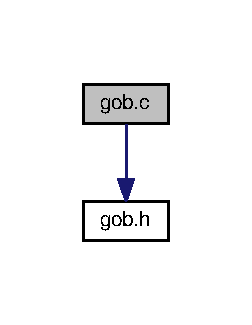
\includegraphics[width=121pt]{gob_8c__incl}
\end{center}
\end{figure}
\subsection*{Functions}
\begin{DoxyCompactItemize}
\item 
void \hyperlink{gob_8c_a45e541c36ac41c90392d01fb39640f5e}{cleanup\+\_\+garbage} (void $\ast$target)
\end{DoxyCompactItemize}


\subsection{Function Documentation}
\hypertarget{gob_8c_a45e541c36ac41c90392d01fb39640f5e}{\index{gob.\+c@{gob.\+c}!cleanup\+\_\+garbage@{cleanup\+\_\+garbage}}
\index{cleanup\+\_\+garbage@{cleanup\+\_\+garbage}!gob.\+c@{gob.\+c}}
\subsubsection[{cleanup\+\_\+garbage}]{\setlength{\rightskip}{0pt plus 5cm}void cleanup\+\_\+garbage (
\begin{DoxyParamCaption}
\item[{void $\ast$}]{target}
\end{DoxyParamCaption}
)}}\label{gob_8c_a45e541c36ac41c90392d01fb39640f5e}
Simply steps through the garbage chain, calling the cleanup function for each node, terminating when N\+U\+L\+L.

The cleanup function could quite simply be set to free(). But it should be set to something otherwise it will do nothing and skip the object, leaking it into memory. In that case it really is your fault for not setting a cleanup function. 
\hypertarget{gob_8h}{\section{gob.\+h File Reference}
\label{gob_8h}\index{gob.\+h@{gob.\+h}}
}
This graph shows which files directly or indirectly include this file\+:\nopagebreak
\begin{figure}[H]
\begin{center}
\leavevmode
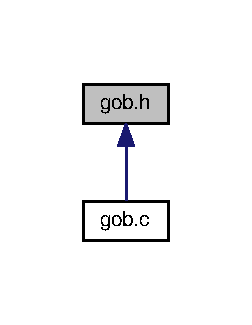
\includegraphics[width=121pt]{gob_8h__dep__incl}
\end{center}
\end{figure}
\subsection*{Data Structures}
\begin{DoxyCompactItemize}
\item 
struct \hyperlink{structraygan__general__object}{raygan\+\_\+general\+\_\+object}
\end{DoxyCompactItemize}
\subsection*{Typedefs}
\begin{DoxyCompactItemize}
\item 
\hypertarget{gob_8h_a206ffc251b8ccefb3e952a12d9afeef9}{typedef struct \\*
\hyperlink{structraygan__general__object}{raygan\+\_\+general\+\_\+object} {\bfseries gob}}\label{gob_8h_a206ffc251b8ccefb3e952a12d9afeef9}

\end{DoxyCompactItemize}
\subsection*{Functions}
\begin{DoxyCompactItemize}
\item 
void \hyperlink{gob_8h_a9d8fa5b2a38077865071ba07a3a5db7c}{cleanup\+\_\+garbage} (void $\ast$)
\end{DoxyCompactItemize}


\subsection{Function Documentation}
\hypertarget{gob_8h_a9d8fa5b2a38077865071ba07a3a5db7c}{\index{gob.\+h@{gob.\+h}!cleanup\+\_\+garbage@{cleanup\+\_\+garbage}}
\index{cleanup\+\_\+garbage@{cleanup\+\_\+garbage}!gob.\+h@{gob.\+h}}
\subsubsection[{cleanup\+\_\+garbage}]{\setlength{\rightskip}{0pt plus 5cm}void cleanup\+\_\+garbage (
\begin{DoxyParamCaption}
\item[{void $\ast$}]{target}
\end{DoxyParamCaption}
)}}\label{gob_8h_a9d8fa5b2a38077865071ba07a3a5db7c}
G\+A\+R\+B\+A\+G\+E C\+O\+L\+L\+E\+C\+T\+I\+O\+N M\+E\+T\+H\+O\+D. this method name could change. but I want to keep it simple.

Simply steps through the garbage chain, calling the cleanup function for each node, terminating when N\+U\+L\+L.

The cleanup function could quite simply be set to free(). But it should be set to something otherwise it will do nothing and skip the object, leaking it into memory. In that case it really is your fault for not setting a cleanup function. 
%--- End generated contents ---

% Index
\newpage
\phantomsection
\addcontentsline{toc}{chapter}{Index}
\printindex

\end{document}
